\documentclass[tikz,border=10pt]{standalone}
\usepackage{tikz}
\usetikzlibrary{shapes.geometric, arrows.meta, positioning, fit, calc, backgrounds, shadows}

% Color Palette (Nature/Science style)
\definecolor{mantisBlue}{RGB}{66, 133, 244}   % Main Process
\definecolor{mantisRed}{RGB}{234, 67, 53}     % Controller/Decision
\definecolor{mantisGreen}{RGB}{52, 168, 83}   % Memory
\definecolor{mantisYellow}{RGB}{251, 188, 5}  % Warning/Critic
\definecolor{mantisGray}{RGB}{240, 240, 240}  % Backgrounds
\definecolor{darkGray}{RGB}{100, 100, 100}

\begin{document}

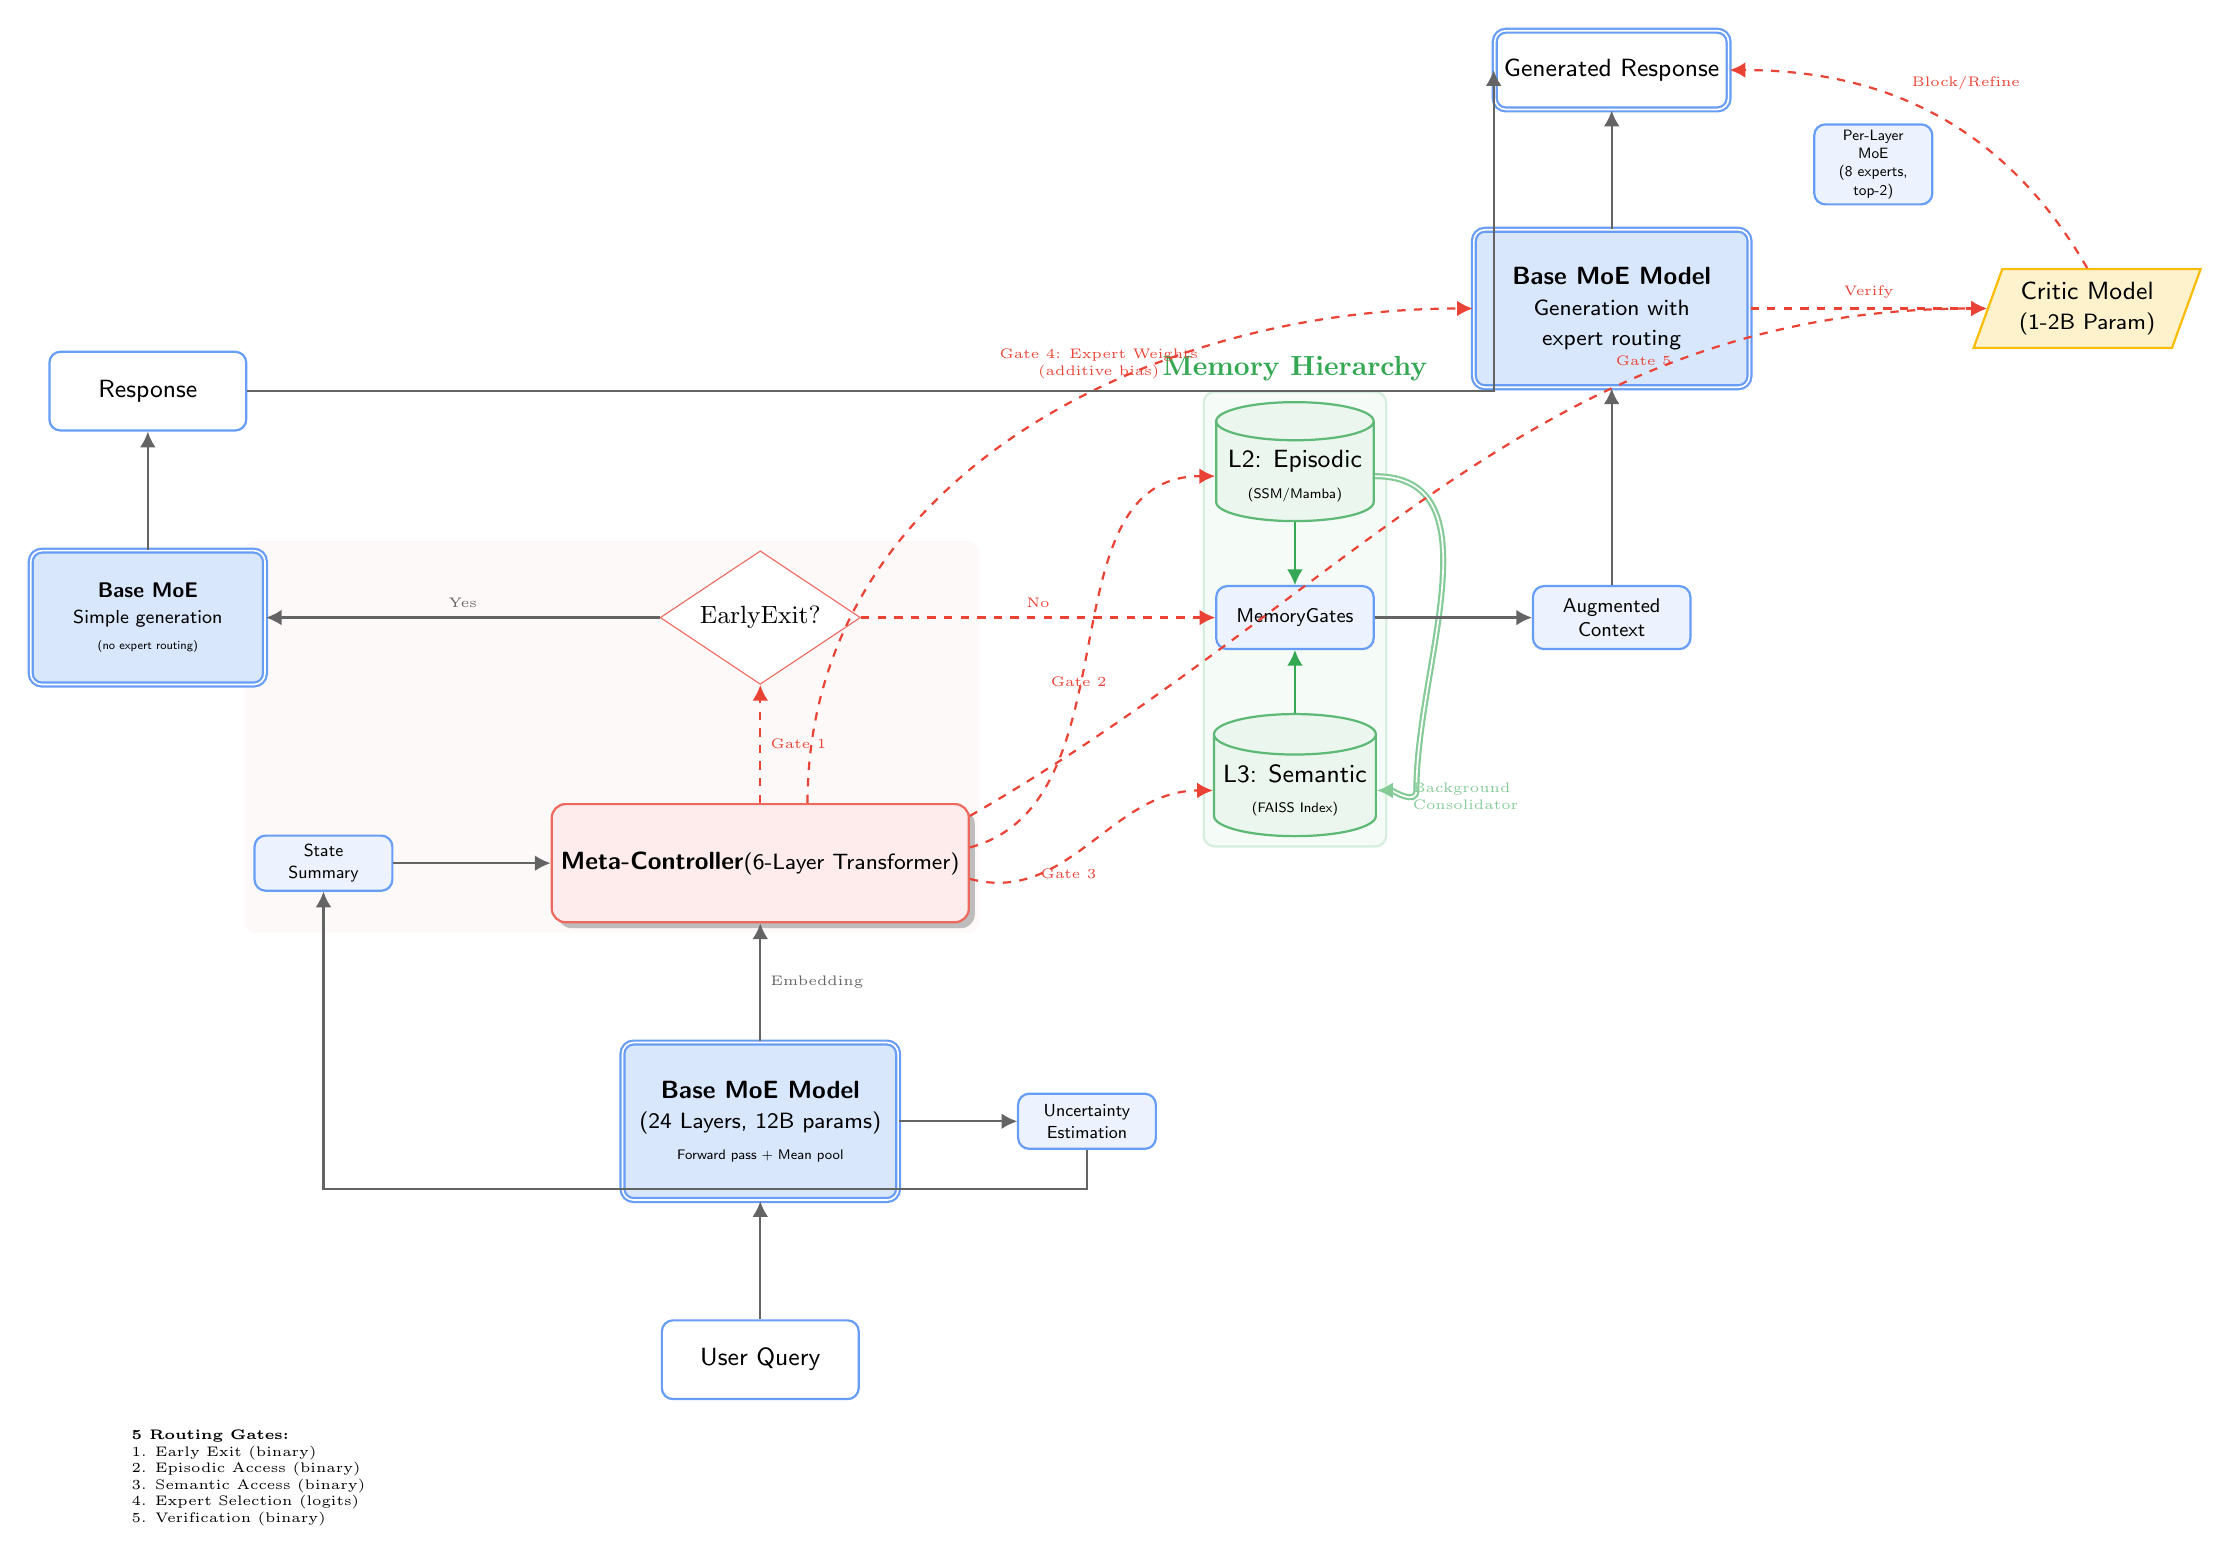
\begin{tikzpicture}[
    node distance=2cm and 2.5cm,
    font=\sffamily\small,
    >={Latex[width=2mm,length=2mm]},
    % Node Styles
    process/.style={
        rectangle,
        rounded corners,
        minimum width=2.5cm,
        minimum height=1cm,
        text centered,
        draw=mantisBlue!80,
        fill=mantisBlue!10,
        thick
    },
    controller/.style={
        rectangle,
        rounded corners=5pt,
        minimum width=3cm,
        minimum height=1.5cm,
        text centered,
        draw=mantisRed!80,
        fill=mantisRed!10,
        thick,
        drop shadow
    },
    memory/.style={
        cylinder,
        shape border rotate=90,
        aspect=0.25,
        minimum width=2cm,
        minimum height=1.5cm,
        text centered,
        draw=mantisGreen!80,
        fill=mantisGreen!10,
        thick
    },
    moe_model/.style={
        rectangle,
        rounded corners,
        minimum width=3.5cm,
        minimum height=2cm,
        text centered,
        draw=mantisBlue!80,
        fill=mantisBlue!20,
        thick,
        double
    },
    decision/.style={
        diamond,
        aspect=1.5,
        minimum width=1.8cm,
        minimum height=1cm,
        draw=mantisRed!80,
        fill=white,
        font=\small
    },
    critic/.style={
        trapezium,
        trapezium left angle=70,
        trapezium right angle=110,
        minimum width=2.5cm,
        minimum height=1cm,
        draw=mantisYellow!100!orange,
        fill=mantisYellow!20,
        thick
    },
    % Connector Styles
    flow/.style={->, thick, darkGray},
    control/.style={->, thick, mantisRed, dashed},
    memory_link/.style={->, thick, mantisGreen},
    consolidation/.style={->, double, thick, mantisGreen!60}
]

% --- Step 1: Query Input & Full Encoding ---

\node (input) [process, fill=white] {User Query};

% Base MoE for encoding (FIRST PASS)
\node (encoder) [moe_model, above=1.5cm of input, align=center] {
    \textbf{Base MoE Model}\\
    {\footnotesize (24 Layers, 12B params)}\\
    {\tiny Forward pass + Mean pool}
};
\draw[flow] (input) -- (encoder);

% Uncertainty estimation
\node (uncertainty) [process, right=1.5cm of encoder, scale=0.7, align=center] {Uncertainty\\Estimation};
\draw[flow] (encoder.east) -- (uncertainty.west);

% --- Step 2: Meta-Controller Routing ---

\node (meta) [controller, above=1.5cm of encoder] {
    \textbf{Meta-Controller}\\
    {\footnotesize (6-Layer Transformer)}
};
\draw[flow] (encoder) -- node[right, font=\tiny] {Embedding} (meta);

% State Summary
\node (state) [process, left=2cm of meta, scale=0.7, align=center] {State\\Summary};
\draw[flow] (uncertainty.south) -- ++(0,-0.5) -| (state.south);
\draw[flow] (state) -- (meta);

% --- Step 3: Routing Decision ---

\node (early_check) [decision, above=1.5cm of meta] {Early\\Exit?};
\draw[control] (meta.north) -- node[right, font=\tiny] {Gate 1} (early_check);

% --- LEFT PATH: Early Exit (uses Base MoE again) ---

\node (simple_gen) [moe_model, left=5cm of early_check, align=center, scale=0.85] {
    \textbf{Base MoE}\\
    {\footnotesize Simple generation}\\
    {\tiny (no expert routing)}
};
\draw[flow] (early_check) -- node[above, font=\tiny] {Yes} (simple_gen);

\node (simple_out) [process, above=1.5cm of simple_gen, fill=white] {Response};
\draw[flow] (simple_gen) -- (simple_out);

% --- RIGHT PATH: Memory + Expert Routing ---

% Memory decision - increased spacing
\node (mem_gate) [process, right=4.5cm of early_check, scale=0.8] {Memory\\Gates};
\draw[control] (early_check) -- node[above, font=\tiny] {No} (mem_gate);

% L2: Episodic Memory - increased spacing
\node (episodic) [memory, above=0.8cm of mem_gate, align=center] {L2: Episodic\\{\tiny (SSM/Mamba)}};
\draw[control] ($(meta.east)+(0, 0.2)$) to[out=15, in=180] node[pos=0.4, above, font=\tiny] {Gate 2} (episodic.west);
\draw[memory_link] (episodic.south) -- (mem_gate.north);

% L3: Semantic Memory - increased spacing
\node (semantic) [memory, below=0.8cm of mem_gate, align=center] {L3: Semantic\\{\tiny (FAISS Index)}};
\draw[control] ($(meta.east)-(0, 0.2)$) to[out=-15, in=180] node[pos=0.4, below, font=\tiny] {Gate 3} (semantic.west);
\draw[memory_link] (semantic.north) -- (mem_gate.south);

% Consolidation - route around to avoid crossing mem_gate
\draw[consolidation] (episodic.east) to[out=0, in=90] ($(semantic.east)+(0.5,0)$) to[out=-90, in=0] node[right, font=\tiny, align=left] {Background\\Consolidator} (semantic.east);

% Augmented context
\node (context) [process, right=2cm of mem_gate, scale=0.8, align=center] {Augmented\\Context};
\draw[flow] (mem_gate) -- (context);

% --- Step 4: Generation with Expert Routing ---

\node (expert_gen) [moe_model, above=2.5cm of context, align=center] {
    \textbf{Base MoE Model}\\
    {\footnotesize Generation with}\\
    {\footnotesize expert routing}
};
\draw[flow] (context) -- (expert_gen);

% Expert weights from meta-controller - routed to avoid crossing boxes
\draw[control] ($(meta.north)+(0.6, 0)$) to[out=90, in=180] node[pos=0.6, above, font=\tiny, align=center] {Gate 4: Expert Weights\\(additive bias)} (expert_gen.west);

% MoE layers (conceptual representation) - moved above to avoid overlap
\node (moe_layers) [process, above right=0.3cm and 0.8cm of expert_gen, scale=0.6, align=center] {Per-Layer\\MoE\\(8 experts,\\top-2)};

% --- Step 5: Verification (Optional) ---

\node (critic) [critic, right=3cm of expert_gen, align=center] {Critic Model\\{\footnotesize (1-2B Param)}};
\draw[control] ($(meta.east)+(0, 0.6)$) to[out=30, in=180] node[pos=0.7, above, font=\tiny] {Gate 5} (critic.west);
\draw[control, dashed] (expert_gen.east) -- node[above, font=\tiny] {Verify} (critic.west);

% --- Final Output ---

\node (output) [process, above=1.5cm of expert_gen, fill=white, double] {Generated Response};
\draw[flow] (expert_gen) -- (output);
\draw[control, dashed] (critic.north) to[out=120, in=0] node[pos=0.6, above right, font=\tiny] {Block/Refine} (output.east);

% Merge early exit path
\draw[flow] (simple_out.east) -| (output.west);

% --- Backgrounds/Grouping ---

\begin{pgfonlayer}{background}
    % Memory System
    \node [fit=(episodic) (semantic) (mem_gate), fill=mantisGreen!5, rounded corners, draw=mantisGreen!20, thick, label={[mantisGreen, font=\bfseries]above:Memory Hierarchy}] {};

    % Meta-Controller decision zone
    \node [fit=(meta) (state) (early_check), fill=mantisRed!3, rounded corners, draw=none] {};
\end{pgfonlayer}

% Legend
\node[font=\tiny, align=left] at (-6.5, -1.5) {
    \textbf{5 Routing Gates:}\\
    1. Early Exit (binary)\\
    2. Episodic Access (binary)\\
    3. Semantic Access (binary)\\
    4. Expert Selection (logits)\\
    5. Verification (binary)
};

\end{tikzpicture}
\end{document}
